\chapter{Superfície (Malha de Triângulos)}
\label{cap_surface}

No InVesalius, a superfície 3D é gerada com base em um modelo segmentado (obtido a partir
da segmentação das imagens). O método utilizado para gerar a superfície é o algoritmo 
\textit{marching cubes}. Resumidamente, o algoritmo transforma os \textit{voxels} das
imagens que foram "empilhadas" e segmentadas em uma malha de polígonos simples - no caso,
triângulos.

Os controles disponíveis para a configuração de superfícies 3D no InVesalius encontram-se
no painel esquerdo do software, dentro do item \textbf{3. Configure a superfície 3D}, opção
\textbf{Propriedades da superfície}.

\begin{figure}[!htb]
\centering
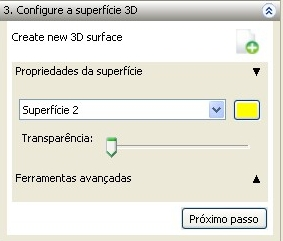
\includegraphics[scale=0.5]{ScreenHunter_23_Jan_23_23_10}
\caption{Configuração de uma superfície 3D}
\label{fig:3d_surface_managment}
\end{figure}


\section{Criando superfícies}

É possível criar uma nova superfície com base em uma máscara de segmentação já existente.
Para isso, no painel esquerdo, dentro do item \textbf{3. Configure a superfície 3D}, clique
no atalho ilustrado na figura \ref{fig:shortcut_new_surface}.

\begin{figure}[!htb]
\centering

\includegraphics[scale=0.18]{object_add_original}
\caption{Atalho para criar uma superfície}
\label{fig:shortcut_new_surface}
\end{figure}

Ao se clicar nesse atalho, uma janela se abre para permitir a configuração da superfície a
ser criada (figura \ref{fig:create_surface_1}). Além de ser possível determinar a qualidade
da superfície a gerar, há opções também para o preenchimento de buracos existentes e para a
seleção da maior região da superfície.

\begin{figure}[!htb]
\centering
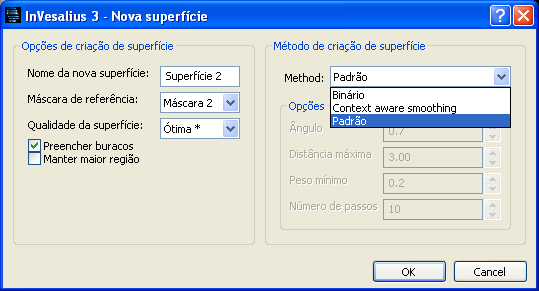
\includegraphics[scale=0.5]{new_surface.png}
\caption{Janela para criação de superfície}
\label{fig:create_surface_1}
\end{figure}

%Existe 2 opções para fechar os buracos existentes e para selecionar a maior região da superfície aonde em muitos 
%casos é útil para remover o suporte ou a mesa do tomografo.

A seleção da maior região pode ser usada, por exemplo, para remover do modelo o suporte ou a
mesa do tomógrafo. A figura \ref{fig:surface_ex1} ilustra um caso com as duas opções
selecionadas: "Preencher buracos" e "Manter maior região".

\newpage

\begin{figure}
  \centering
  \subfloat[Frente]{\label{fig:__1}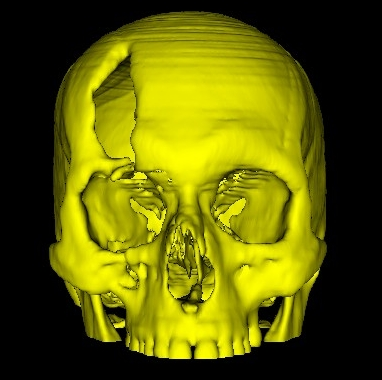
\includegraphics[width=0.338\textwidth]{ScreenHunter_48_Jan_23_23_34}}                
  \subfloat[Baixo]{\label{fig:__1}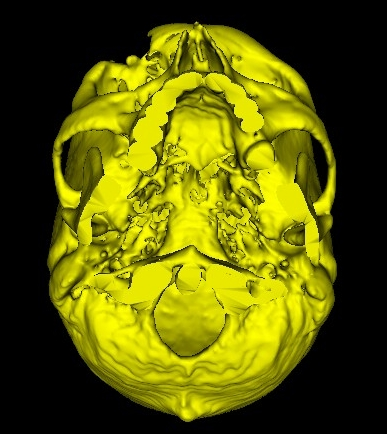
\includegraphics[width=0.3\textwidth]{ScreenHunter_50Jan232334}}
  \caption{Superfície com região maior selecionada e com buracos preenchidos}
  \label{fig:surface_ex1}
\end{figure}


Já a figura \ref{fig:surface_ex2} mostra o mesmo caso sem essas opções selecionadas. Observa-se o
suporte do tomógrafo e a superfície aberta.


\begin{figure}
  \centering
  \subfloat[Frente]{\label{fig:__2}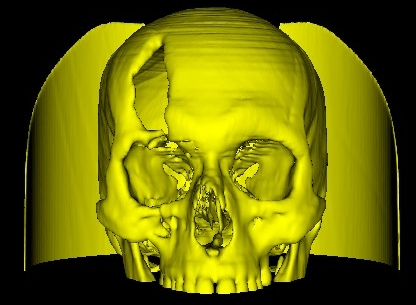
\includegraphics[width=0.371\textwidth]{ScreenHunter_52Jan232335}}                
  \subfloat[Baixo]{\label{fig:__2}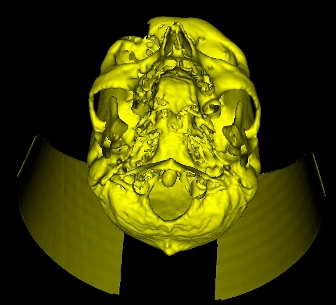
\includegraphics[width=0.3\textwidth]{ScreenHunter_53Jan232336}}
  \caption{Superfície sem a seleção da maior região e com buracos abertos}
  \label{fig:surface_ex2}
\end{figure}

O item \textbf{Método de criação de superfície} tem as seguintes opções, \textbf{"Binário"}, \textbf{"Context aware smoothing"} e \textbf{"Padrão}, podemos visualizar um exemplo de superfície a partir dos 3 métodos na figura \ref{fig:surf_method}. 

O método \textbf{binário}, tem como partida a máscara que foi segmentada, sendo a região selecionada como 1 e o restante 0. Como existem somente 2 valores, as curvas na superfície que o algoritmo gera são abruptas ou popularmente conhecida como "degraus".

No método \textbf{Context aware smoothing}, inicialmente a superfície é gerada a partir do método binário, mas em seguida é executado o algoritmo "Context aware smoothing" para suavizar a superfície resultante e evitar os "degraus" na mesma. Neste passo é requerido 4 valores, que serão apresentados a seguir.

O \textbf{ângulo}, nesse caso será formado entre 2 normais de triângulos adjacentes, que \textbf{caso esteja acima do valor} definido no campo ângulo, o triângulo é elegido para ser o ponto de partida da suavização, a faixa de valor é de 0 até 1, sendo $0^\circ$ e $90^\circ$ respectivamente. A \textbf{distância máxima} é o raio a partir dos triângulos elegidos no passo anterior, que será utilizada como limite de suavização. O \textbf{peso mínimo} é o quanto de suavização será aplicado nas áreas que estão fora do raio determinado anteriormente. O \textbf{número de passos} é quantas vezes o algoritmo vai executar. 

O método \textbf{padrão} é ativo \textbf{somente quando não existir edição manual na máscara}, os pixeis da imagem original que estão sob a máscara é utilizado para a geração de superfície, como normalmente imagens de tomografia ou ressonância possui vários níveis de cinza, é gerada uma superfície com curvas mais suaves.

\begin{figure}[!htb]
  \centering
  \subfloat[Binário]{\label{fig:surf_binary}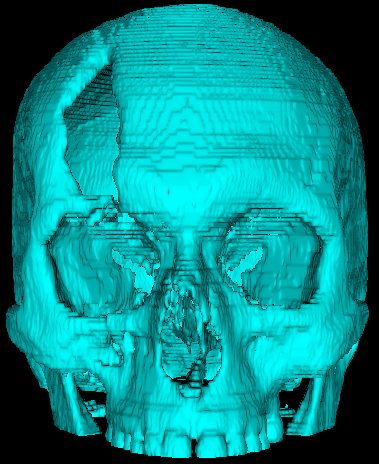
\includegraphics[width=0.33\textwidth]{binary.png}}                
  \hfill
  \subfloat[Context aware]{\label{fig:surf_context}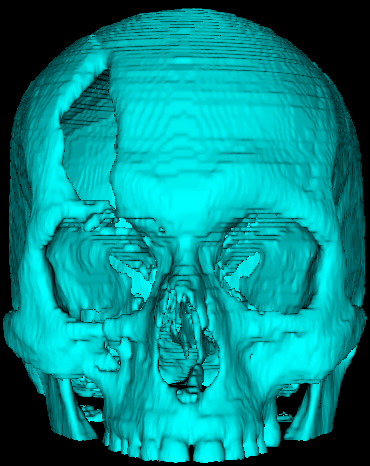
\includegraphics[width=0.32\textwidth]{context.png}}	
  \hfill  
  \subfloat[Padrão]{\label{fig:surfa_default}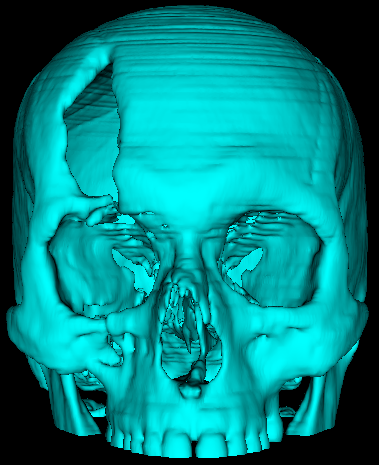
\includegraphics[width=0.332\textwidth]{default.png}}
  \caption{Superfícies geradas por diferentes métodos }
  \label{fig:surf_method}
\end{figure}



\section{Transparência}

É possível visualizar uma superfície com transparência. Para isso, primeiro selecione a
superfície por meio da lista de seleção, dentro do item \textbf{3. Configure a superfície 3D}, opção
\textbf{Propriedades da superfície} (figura \ref{fig:select_surface}).

\begin{figure}[!htb]
\centering

\includegraphics[scale=0.6]{select_surface}
\caption{Seleção de superfície}
\label{fig:select_surface}
\end{figure}

Em seguida, para determinar o nível de transparência que a superfície selecionada receberá, arraste
o controle deslizante ilustrado na figura \ref{fig:select_transparency}. Quanto mais para a direita
o controle, maior será a transparência aplicada.

\begin{figure}[!htb]
\centering
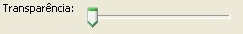
\includegraphics[scale=0.5]{transparency}
\caption{Seleção de nível de transparência}
\label{fig:select_transparency}
\end{figure}

A figura \ref{fig:model_transparency} ilustra a visualização de duas superfícies: uma mais externa
(esverdeada) e outra mais interna (amarelada). A superfície mais externa aparece com a transparência
aumentada.

\begin{figure}[!htb]
\centering
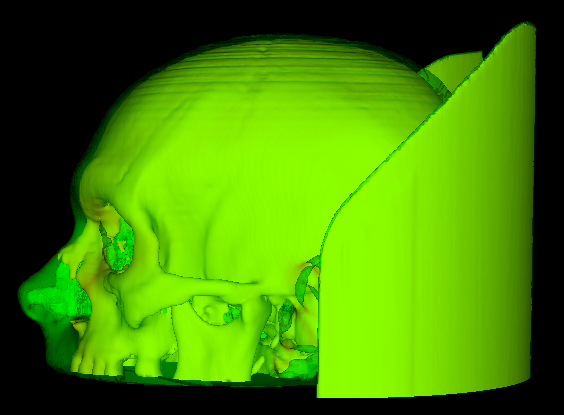
\includegraphics[scale=0.3]{transparency_2}
\caption{Superfícies com nível alterado de transparência}
\label{fig:model_transparency}
\end{figure}

\newpage

\section{Cor}

A cor de uma superfície também pode ser alterada. Selecione a superfície (reveja a figura
\ref{fig:select_surface}) e, em seguida, clique no botão ao lado da superfície selecionada. A figura
\ref{fig:change_surface_color} ilustra o botão, também localizado no item \textbf{3. Configure a
superfície 3D}, opção \textbf{Propriedades da superfície}.

\begin{figure}[!htb]
\centering

\includegraphics[scale=0.6]{button_select_color}
\caption{Botão para alteração de cor}
\label{fig:change_surface_color}
\end{figure}

Uma janela de seleção de cores se abre (figura \ref{fig:button_select_color}). Selecione a cor
desejada e clique no botão \textbf{OK}.

\begin{figure}[!htb]
\centering
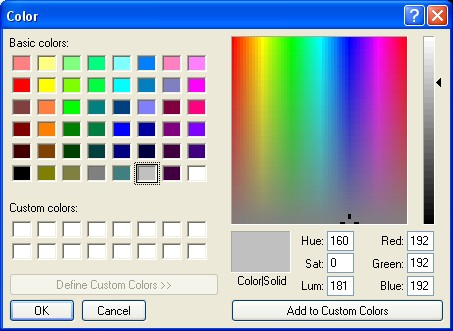
\includegraphics[scale=0.4]{ScreenHunter_33Dec311142}
\caption{Opções de cor}
\label{fig:button_select_color}
\end{figure}

\section{Separando regiões desconexas}

Para separar regiões da superfície que se encontram desconexas, é necessário clicar na opção
\textbf{Ferramentas avançadas}, dentro do item \textbf{3. Configure a superfície 3D}. Veja a
figura \ref{fig:advanced_tools}.

\begin{figure}[!htb]
\centering
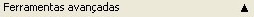
\includegraphics[scale=0.4]{ferramentas_avancadas}
\caption{Atalho para ferramentas avançadas}
\label{fig:advanced_tools}
\end{figure}

\newpage

Um menu com as opções disponíveis será exibido, como ilustra a figura
\ref{fig:advanced_tools_expanded}.

\begin{figure}[!htb]
\centering
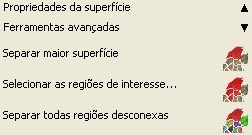
\includegraphics[scale=0.5]{exract_region}
\caption{Ferramentas avançadas}
\label{fig:advanced_tools_expanded}
\end{figure}

\subsection{Separar maior superfície}

A opção \textbf{Separar maior superfície} seleciona, automaticamente, somente a região
desconexa que contém maior volume. Para realizar a operação, basta clicar no atalho
que a figura \ref{fig:short_connectivity_largest} ilustra. É criada uma nova superfície
resultante da operação.

\begin{figure}[!htb]
\centering
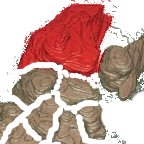
\includegraphics[scale=0.2]{connectivity_largest}
\caption{Atalho para separação da maior região desconexa}
\label{fig:short_connectivity_largest}
\end{figure}

Como exemplo, a figura \ref{fig:extract_most_region_1} mostra um caso antes da separação
da maior região.

\begin{figure}[!htb]
\centering
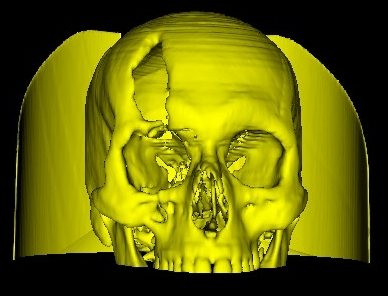
\includegraphics[scale=0.3]{extract_most_region_1}
\caption{Superfícies desconexas}
\label{fig:extract_most_region_1}
\end{figure}

Na figura \ref{fig:extract_most_region2}, observa-se a superfície com a maior região
desconexa separada.

\begin{figure}[!htb]
\centering
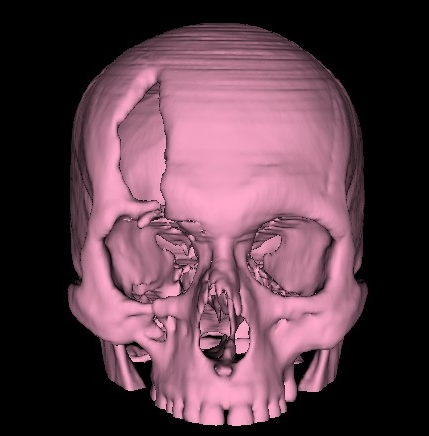
\includegraphics[scale=0.3]{extract_most_region2}
\caption{Maior região separada}
\label{fig:extract_most_region2}
\end{figure}

\newpage

\subsection{Selecionar as regiões de interesse}

Outra modalidade de seleção se dá pela opção \textbf{Selecionar as regiões de interesse...}.
Para ativá-la, o usuário deve clicar sobre o botão ilustrado na figura
\ref{fig:short_connectivity_manual}. Em seguida, basta clicar sobre as regiões desconexas
da superfície que se pretende selecionar.

\begin{figure}[!htb]
\centering
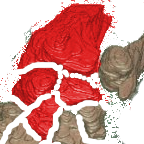
\includegraphics[scale=0.2]{connectivity_manual}
\caption{Atalho para seleção de regiões de interesse}
\label{fig:short_connectivity_manual}
\end{figure}

No exemplo da figura \ref{fig:extract_most_region3}, foram selecionados o crânio e a parte
direita do suporte do tomógrafo.

\begin{figure}[!htb]
\centering
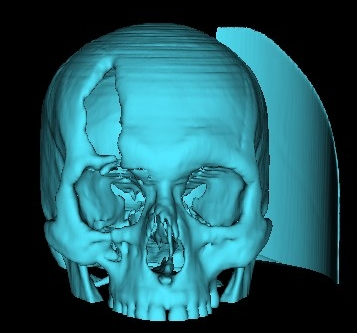
\includegraphics[scale=0.35]{extract_most_region3}
\caption{Exemplo de regiões de interesse selecionadas}
\label{fig:extract_most_region3}
\end{figure}


\subsection{Separar todas regiões desconexas}

É possível, também, separar automaticamente \textit{todas} as regiões desconexas. Para
isso, basta clicar no botão ilustrado pela figura \ref{fig:connectivity_split_all}, que
representa a opção \textbf{Separar todas regiões desconexas}.

\begin{figure}[!htb]
\centering
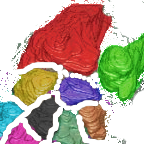
\includegraphics[scale=0.2]{connectivity_split_all}
\caption{Atalho para separação de todas as regiões desconexas}
\label{fig:connectivity_split_all}
\end{figure}

A figura \ref{fig:extrac_most_region_4} mostra um exemplo.

\begin{figure}[!htb]
\centering
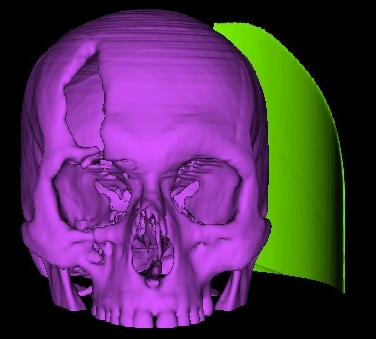
\includegraphics[scale=0.3]{extrac_most_region_4}
\caption{Exemplo de separação de todas as regiões desconexas}
\label{fig:extrac_most_region_4}
\end{figure}

